\section{Theory}\label{sec:theory}

The propositions below explain why the sequence should work, state what the lock does and does not guarantee, and say how much of the frame-count equation is derived and how much is calibrated. Where a statement could not be proved it is stated as a conjecture with the evidence for it. Proposition~\ref{prop:blend} is used to read the measured transient ratios, Proposition~\ref{prop:frames} gives the frame count of Eq.~\ref{eq:frames}, and Proposition~\ref{prop:lock} is the statement about phase continuity that distinguishes the lock from the induction.

\subsection{Transient intensity of a shifted pattern}

\begin{proposition}\label{prop:blend}
Consider a single trap read in the blend model of Section~\ref{sec:problem}, with a flat input amplitude over $n$ pixels along one axis, and two consecutive holograms $\phi^{(s)}$ and $\phi^{(s+1)}=\phi^{(s)}+2\pi\delta\,j/n$ that display the same pattern shifted by $\delta$ Fourier units, with $\phi_j^{(s)}-\Delta_j^{(s)}$ constant over the pixels (a hologram of one trap in phase at all pixels). At the half-way instant $\alpha=\tfrac12$, read at the position $\delta/2$ from the trap of frame $s$, the intensity as a fraction of the frame's own intensity is
\begin{equation}
\frac{I(s,\tfrac12)}{I(s)}=\operatorname{sinc}^2\!\Big(\frac\delta2\Big),\qquad \operatorname{sinc}x=\frac{\sin\pi x}{\pi x},\label{eq:sinc}
\end{equation}
in the limit of many pixels, and it equals $0.9$ at the shift $\delta_{0.9}=\deltaNine{}$ Fourier units.
\end{proposition}
\begin{proof}
Let $j$ run over $n$ pixels centred on zero. The blend field is $\tfrac12e^{i\phi_j^{(s)}}(1+e^{2\pi i\delta j/n})$. The read-out at the shifted position adds the delay $\pi\delta j/n$ to the trap's own delay, so the amplitude is $\frac1n\sum_j\tfrac12e^{i(\phi_j^{(s)}-\Delta_j^{(s)})}\big(e^{-i\pi\delta j/n}+e^{+i\pi\delta j/n}\big)=\frac1n\sum_je^{i(\phi_j^{(s)}-\Delta_j^{(s)})}\cos(\pi\delta j/n)$. With the phase constant the sum is $\frac1n\sum_j\cos(\pi\delta j/n)\to\int_{-1/2}^{1/2}\cos(\pi\delta u)\,du=\operatorname{sinc}(\delta/2)$, and the intensity is its square. The value $\delta_{0.9}$ is the root of $\operatorname{sinc}^2(\delta/2)=0.9$, found by bisection.
\end{proof}

The closed form is a reference for a single trap. In a multi-trap hologram the other traps change between frames as well, and the lowest moving trap can lie below the single-trap value. Two comparisons show how the measurements stand against it. At the peak step of the acceptance task, \accPeakStep{} Fourier units, Eq.~\ref{eq:sinc} gives \sincAcc{}, and the measured lowest transient ratio of the sequence is \accBTransMean{} on average. At the step bound of the sequence, \claimStepFu{} Fourier units, it gives \sincClaim{}, and the lattice moves of Table~\ref{tab:long}, at peak steps of \longAPeak{} and \longBPeak{} Fourier units, measure medians of \longAMed{} and \longBMed{}. The bound of the sequence is therefore not the shift at which the single-trap form reaches $0.9$, which is \deltaNine{} Fourier units, but a more conservative step. The close agreement of \sincAcc{} with the measured mean on the acceptance task is partly a coincidence of one case: the closed form ignores the other traps, the finite input beam and the weights, and the sequence is below it on the long moves.

\subsection{Frames and the step bound}

\begin{proposition}\label{prop:frames}
For the minimal-jerk profile the largest shift between consecutive frames of a trap that travels $L$ Fourier units in $S$ intervals is $\delta_{\max}\approx\frac{15}{8}L/S$, and a step bound $\delta_{\mathrm{claim}}$ requires $S\ge\frac{15}{8}L/\delta_{\mathrm{claim}}$ intervals; the number of frames of a sequence, and so its cost, grows linearly with the length of the move.
\end{proposition}
\begin{proof}
The profile of Eq.~\ref{eq:minjerk} has $h'(\tau)=30\tau^2(1-\tau)^2$, which is maximal at $\tau=\tfrac12$ with value $\tfrac{30}{16}=\tfrac{15}{8}$. For large $S$ the shift between frames $s$ and $s+1$ is $L(h(\tfrac{s+1}S)-h(\tfrac sS))\approx Lh'(\tfrac sS)/S\le\frac{15}8L/S$. Solving $\frac{15}8L/S\le\delta_{\mathrm{claim}}$ for $S$ gives the bound.
\end{proof}

For the moves of the paper, Eq.~\ref{eq:frames} gives \accFramesForMove{} frames for the acceptance move, \longAFrames{} and \longBFrames{} frames for the two lattice moves and \cTenFrames{} frames for the longest move of the sort (Fig.~\ref{fig:theory}b). The acceptance task is run with \parFrames{} frames, fewer than the bound, because the bound is sufficient and not necessary: at the step of \accPeakStep{} Fourier units the sequence still keeps the transient ratio at \accBTransMean{}. The value of $\delta_{\mathrm{claim}}$ is a calibration. It is the peak step at which the lowest moving trap of the sort of the studio's rearrangement case reached $0.9$ in a pilot with one seed; the closed form of Proposition~\ref{prop:blend} alone would permit a step of \deltaNine{} Fourier units for a single trap. The calibration has a consequence that Section~\ref{sec:results} measures: the bound is a rule that holds on most seeds and not on all.

\begin{figure}[t]
\centering
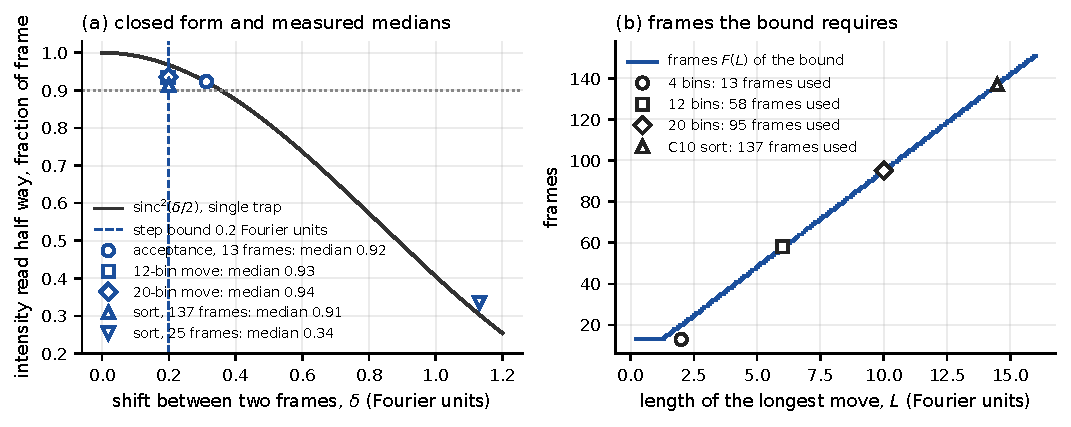
\includegraphics[width=\textwidth]{fig-theory.pdf}
\caption{Theory of the transient intensity. (a) Closed form $\operatorname{sinc}^2(\delta/2)$ of the intensity of a single trap read half way between two frames shifted by $\delta$ Fourier units, with the step bound of the sequence and the median transient minimum ratio measured at the peak steps of the acceptance task (13 frames), the two lattice moves and the sort. (b) Frames that the bound requires against the length of the move, with the frame counts used in the experiments marked.}
\label{fig:theory}
\end{figure}

Figure~\ref{fig:theory} shows both statements. Panel (a) shows that the closed form falls slowly at first, so a small shift costs little and the bound on the step is what keeps the single-trap intensity above $0.9$; the measured points lie below the curve on the long moves, which is the effect of the other traps and of the seeds that fail. It does not show the effect of the weights or the locks, which are measured and not derived. Panel (b) shows that the frame count rises linearly with the move, so the longest rearrangement move needs several times the frames of the acceptance move, which is the practical limit of the method discussed in Section~\ref{sec:discussion}.

\subsection{What the lock guarantees about the phase}

\begin{proposition}\label{prop:lock}
Let $\theta_m(s)$ be the prescribed phase of trap $m$, $\psi_m(s)$ its achieved phase $\arg V_m$ at frame $s$, and $\varepsilon_m(s)=\operatorname{wrap}(\psi_m(s)-\theta_m(s))$ the residual of the iteration. Then
\begin{equation}
\big|\operatorname{wrap}\big(\psi_m(s+1)-\psi_m(s)\big)\big|\le\big|\theta_m(s+1)-\theta_m(s)\big|+|\varepsilon_m(s)|+|\varepsilon_m(s+1)|,\label{eq:lockbound}
\end{equation}
and the largest phase step of Eq.~\ref{eq:phasestep} is at most $\dot\theta_{\max}+2\max_{m,s}|\varepsilon_m(s)|$. With held phases, $\theta_m(s)$ is constant, $\Theta\le2\max|\varepsilon|$, and so $\max|\varepsilon|\ge\Theta/2$.
\end{proposition}
\begin{proof}
Write $\psi_m(s)=\theta_m(s)+\varepsilon_m(s)$ modulo $2\pi$. The wrapped difference of two sums is the wrapped sum of the wrapped differences, and the triangle inequality on the circle gives Eq.~\ref{eq:lockbound}. The second statement follows by taking the maximum and using Eq.~\ref{eq:phasebound}. With held phases the first term of the right-hand side is zero, so $\Theta\le2\max|\varepsilon|$.
\end{proof}

Two consequences follow. First, under the lock the phase step is controlled by two quantities, a prescribed one that the user sets and a residual that the iteration leaves, and the residual shrinks as the weighted iteration converges; without the lock there is no prescribed quantity and no control on the step, only the empirical smallness of the change that the induction of Kim et al.\ assumes. Second, the measured step of the sequence on the acceptance task, \accBStepMax{} rad with held phases, is therefore at most twice the largest residual, and by the last statement of the proposition the largest residual phase error over the moving traps and frames of at least one seed is at least \fpeval{round(\accBStepMax/2,3)} rad. The lock does not remove the phase step; it reduces it to the residual of the iteration. This is the statement that Section~\ref{sec:ablation} tests by removing the lock.

\begin{conjecture}\label{conj:phasepath}
When the sequence misses the intensity floor on a long move with the frames of Eq.~\ref{eq:frames}, the cause is the phase path that the end phases prescribe, not the number of frames or the number of iterations per frame.
\end{conjecture}
The evidence is that the seeds that miss the floor on the lattice moves stay below it when the frames are doubled: with the frames of the bound the failing seeds reach \longFailList{}, and with twice the frames \longTwiceList{}. The conjecture would be refuted by a seed that misses the floor with the frames of the move and reaches it with more frames or iterations; the data of this paper contain none. The conditions under which the end phases from the phase-fixed weighted algorithm give a good path are not characterized.
